\section{\method{} with a critic: Stochastic value gradients variants}
\label{sec:method}
We now introduce two SVG-based actor-critic variants, which differentiate the chain itself, avoiding the noise factor $\varepsilon_{k,i}/\sigma_k$ in \methodGRPO{}. Because the terminal reward provides no differentiable path (\S\ref{sec:estimators}), both variants learn a differentiable critic $V_\phi$ for the intermediate-state value~(\ref{eq:value}) and ascend it through one transition. They differ in critic resolution: \methodSVGScalar{} predicts one value per state while \methodSVGTwoD{} predicts one value per state and position.
\subsection{The pathwise update}
\label{sec:pathwise}
\paragraph{Transition-wise value-gradient decomposition.}
The true value $V_k^*(y_k)$ summarizes the expected reward of all continuations from $y_k$. Unrolling the standard stochastic value-gradient (SVG) recursion \citep{heess2015svg} then decomposes the policy gradient into transition-wise contributions. Temporarily assigning transition $k$ its own parameter copy $\theta_k$, tied across steps after differentiation gives $\nabla_\theta J=\sum_{k=2}^{K}\partial J/\partial\theta_k$ and:
\begin{equation}
\frac{\partial J}{\partial\theta_k}=\mathbb E_{y_{k-1},\,\varepsilon_k}\big[\nabla_{\theta_k}V_k^*(y_k)\big],\qquad \nabla_{\theta_k}V_k^*(y_k)
=\alpha_k\lambda_{k-1}\nabla_{y}V_k^*(y_k)\frac{\partial\hat x_{k-1}}{\partial\theta_k},
\label{eq:pw_exact}
\end{equation}\eqalias{eq:chainrule}
Sampling one transition consequently avoids back-propagation through the full chain. Gaussian integration by parts shows that this expression has the same expectation as its score-function counterpart (Appendix~\ref{app:pw_derivation}). At coordinate $(k,i)$, the score-function factor is $V_k^*(y_k)\varepsilon_{k,i}/\sigma_k$, which is noisy at every coordinate, whereas the pathwise factor is $\partial V_k^*(y_k)/\partial y_{k,i}$, which vanishes wherever the value is locally insensitive.

\paragraph{Single-transition actor update.}
We sample $k\sim\mathcal U(\mathcal W)$ from a window
$\mathcal W=\{k_{\rm lo},\dots,k_{\rm hi}\}$ and use $\hat g_{\rm PW}=\nabla_\theta V_\phi(y_k)$. With an exact critic, its expectation is the window-averaged transition gradient. We use the middle of the chain, excluding early states with nearly flat values and late states whose outcomes are nearly determined. 

\begin{figure}[t]
\centering
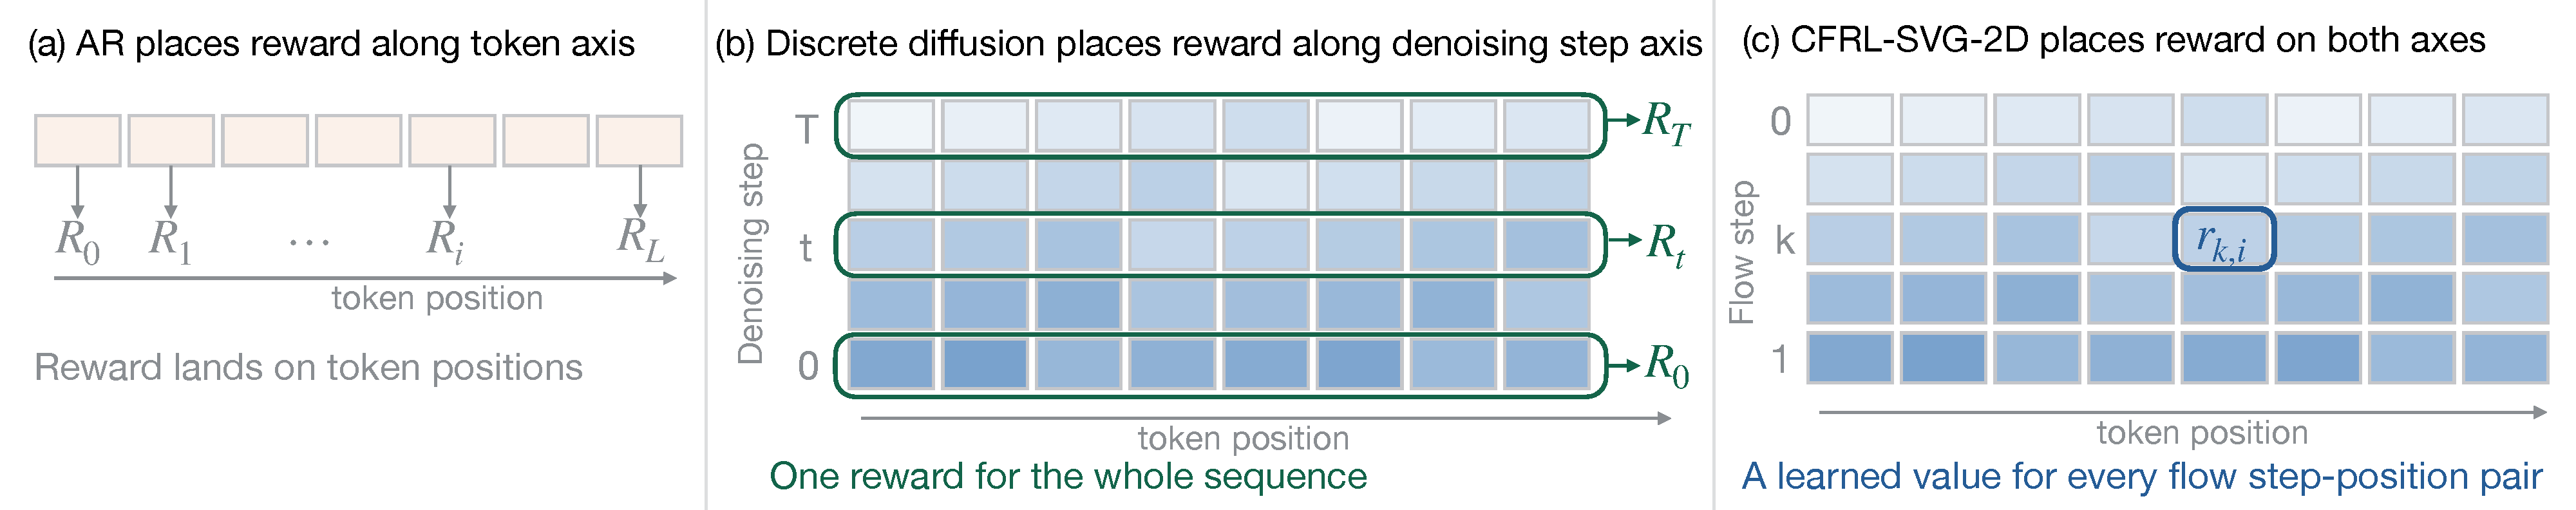
\includegraphics[width=\textwidth]{figures/flow-rl-figure1.pdf}
\caption{Where the reward lands: (a) along the token axis in an AR model; (b) along the denoising-step axis in RL for discrete diffusion; (c) in \method{}-2D the value is indexed by both, $R_{k,i}$ for flow step $k$ and position $i$, each an estimate of the whole response's outcome as read at position $i$, pooled into the actor's objective $V_\phi$.}
\label{fig:mechanism}
\end{figure}

\subsection{The critic: one value per state, or per state and position}
\label{sec:critic}\label{sec:jpc_scalar}\label{sec:jpc_2d}
Predicting success from a noisy state requires anticipating its decoded output, which the denoiser already does. The critic therefore uses a copy $\hat X_\phi$ of the denoiser to map $(y_k, \tilde t_k)$ to per-position features $f_i(y_k)=\hat X_\phi(y_k,\tilde t_k)_i\in\mathbb R^d$, evaluated without guidance. An MLP head $h_\phi$ then converts these features into a value in one of two orders:
\begin{alignat}{2}
&\text{\methodSVGScalar{}:}&\quad V_\phi(y_k)&=h_\phi\big(\tfrac1{|\mathcal G|}\textstyle\sum_{i\in\mathcal G}f_i(y_k),\,\tilde t_k\big),
\label{eq:critic1d}\\
&\text{\methodSVGTwoD{}:}&\quad V_\phi(y_k)&=\tfrac1{|\mathcal G|}\textstyle\sum_{i\in\mathcal G}R_{k,i}, \qquad R_{k,i}=h_\phi\big(f_i(y_k),\tilde t_k\big).
\label{eq:critic2d}
\end{alignat}\eqaliasprev{eq:feat}
A flow model jointly refines all positions over \(K\) steps, giving credit two axes: \emph{when} along the flow and \emph{where} along the sequence (Figure~\ref{fig:mechanism}). Existing diffusion and flow RL methods treat each full-sequence state as an action indexed only by the denoising step \citep{liu2025flowgrpo,xue2025dancegrpo}, as do \method{}-GRPO and \methodSVGScalar{}. In contrast, \methodSVGTwoD{} indexes value by both step and position. Both SVG variants ascend the pooled value and differ only in whether features are pooled before or after the value head. This order determines the signal assigned to each position $i$: $\sum_{j}(\partial V_\phi/\partial f_j)(\partial f_j/\partial y_{k,i})$, where
\begin{equation}
\text{head after the mean: }\ \frac{\partial V_\phi}{\partial f_j}=\frac{\nabla h_\phi(\bar f)}{|\mathcal G|}\ \ \forall j,\qquad \text{head before the mean: }\ \frac{\partial V_\phi}{\partial f_j}=\frac{\nabla h_\phi(f_j)}{|\mathcal G|},
\label{eq:headgrad}
\end{equation}
with $\bar f$ the mean feature and $\nabla h_\phi$ the gradient with respect to its feature input. Mean-then-head applies the head's slope at $\bar f$ to every position, whereas head-then-mean applies its slope at each position's own feature, providing position-specific directions for increasing predicted success. The updates may be similar for a fixed policy and batch because both critics use the same features and outcome labels, but they diverge as the policy moves and the head is refit. Moreover, mean-then-head compresses all positions through the bottleneck $\bar f$; it can equal a mean of per-position readings only when the head is affine (Proposition~\ref{prop:additive}).


\paragraph{Supervision without token labels.}
Both critics are trained on intermediate rollout states using the corresponding terminal outcome $r$; the 2D critic minimizes
\begin{equation}
\mathcal L_{\rm 2D}(\phi)=\tfrac12\,\mathrm{BCE}\big(V_\phi(y_k),r\big)+\tfrac12\,\tfrac1{|\mathcal G|}\textstyle\sum_{i\in\mathcal G}\mathrm{BCE}\big(R_{k,i},r\big),
\label{eq:critic2d_loss}
\end{equation}\eqalias{eq:bce}
while the scalar critic only minimizes the first term. The second calibrates each reading individually; without it the field is constrained only through its mean. One reason to expect the field to stay a usable target \emph{under the refit}: a head on the mean is one function of one vector, which the actor can raise by moving that vector wherever the head reads success, whereas a rise of the pooled field has to be carried by $|\mathcal G|$ readings that the refit keeps calibrated. Without the refit either critic is exploited (\S\ref{sec:exp_2d}). $R_{k,i}$ is not a verifier of token $i$: every reading attends over the whole state and predicts the outcome of the whole response, and within a failed response the readings barely tell wrong positions from right ones (Appendix~\ref{app:critic_maps}). What the field changes is the behaviour of the update under joint training (\S\ref{sec:exp_2d}), not the localisation of errors.

\subsection{Training the critic with the policy}
\label{sec:joint}
The critic is pre-trained on rollouts of the initial policy, copy and head together, and Algorithm~\ref{alg:jpc} then refits it after every actor step: the head only, on a replay buffer of the states that fresh rollouts reach at the top of the window, where the state determines the outcome best. The copy stays frozen (\S\ref{sec:exp_critic}). If the critic's AUC on the newest buffer states falls below a floor, the head takes extra steps before the actor moves again. Both networks are trained under the sampler that will be deployed, since a different sampler is a different chain with different values (Appendix~\ref{app:joint_details}).

\begin{algorithm}[t]
\caption{\method{} with a critic, (\ref{eq:critic1d}) or (\ref{eq:critic2d}); symbols in Appendix~\ref{app:details}}
\label{alg:jpc}
\small
\begin{algorithmic}[1]
\REQUIRE SFT policy $\hat X_\theta$; pre-trained critic $V_\phi$ (frozen copy $\hat X_\phi$, trainable head $h_\phi$); verifier $r$; sampler $(\gamma,K)$; window $\mathcal W=\{k_{\rm lo},\dots,k_{\rm hi}\}$; replay buffer $\mathcal B$ holding the newest $N_{\mathcal B}$ states
\FOR{iteration $=1,\dots,T$}
  \STATE \textbf{Actor.} For $B$ prompts and one $k\sim\mathcal U(\mathcal W)$: roll out to $y_{k-1}$ without gradients, compute $y_k$ from $y_{k-1}$ with gradients, and set $\theta\leftarrow\theta+\eta_\theta\,\mathrm{AdamW}\big(\nabla_\theta\frac1B\sum_{b}V_\phi(y_{k,b})\big)$ (clipped, $\eta_\theta$ decays) 
  \STATE \textbf{Buffer.} Roll out $B$ fresh prompts to the end, decode, verify; push each $(y_{k_{\rm hi}},r)$ into $\mathcal B$
  \STATE \textbf{Critic.} $m_{\rm c}$ head steps $\phi\leftarrow\phi-\eta_\phi\,\mathrm{AdamW}(\nabla_\phi\mathcal L_{\rm 2D})$ on minibatches of $B'$ states of $\mathcal B$; every $n_q$ iterations, $m'_{\rm c}$ more if the AUC of $V_\phi$ on the newest $N_q$ states is below $a_0$ \hfill (eq.~\ref{eq:critic2d_loss})
\ENDFOR
\end{algorithmic}
\end{algorithm}

\paragraph{Amortising the reward improvements into the model.}
\label{sec:loop}
The reward improvement of the SVG variants is tied to their training chain. An optional amortisation step transfers it to other samplers through the model's supervised objective, which trains the denoiser across all times $t$. Each round samples responses from the policy on a pool of unlabelled prompts, retains distinct verified responses, and fine-tunes the model with ELF's original loss (Algorithm~\ref{alg:loop}, Appendix~\ref{app:loop}). With the RL policy as the sampler, this is rejection-sampling fine-tuning \citep{yuan2023rft} corresponding to an EM M-step whose reward lower bound is tight at the current model (Proposition~\ref{prop:em}). Because prompts without accepted responses provide no training signal, improvement depends on pool coverage. The 2D critic can increase coverage by scoring chains through their least confident position, $\min_{i}R_{k,i}$, pruning weak chains, and guiding intermediate states before decoding. This permits pool generation with a cheaper chain, assuming the critic's ranking transfers to its states (Appendix~\ref{app:joint_details}).
